\documentclass[11pt]{article}
\usepackage{mathptmx}
\usepackage{verbatim}
\usepackage[margin=1.25in]{geometry}
\usepackage{graphicx}
\usepackage{color}
\usepackage{url}
\usepackage[colorlinks,
            bookmarks=true,
            hyperindex,
            linkcolor={blue},
            pdftitle={YURT Operations Manual}]{hyperref}

\newsavebox{\notebox}
\newenvironment{note}[1][Note]{\begin{lrbox}{\notebox}%
    \begin{minipage}{0.9\columnwidth}\textcolor{red}{\textbf{#1}:~}}%
    {\end{minipage}\end{lrbox}\begin{center}\setlength{\fboxsep}{8pt}%
    \fbox{\usebox{\notebox}}\end{center}}


% \newenvironment{note}[1][Note]{%
%   \begin{center}\setlength{\fboxsep}{10pt}
%   \framebox\bgroup\begin{minipage}{0.9\columnwidth}\textbf{#1}:~}%
%   {\end{minipage}\egroup\end{center}}


%{\textbf{#1}}{}

\newcommand{\yurt}{YURT}
\newcommand{\cmd}[1]{\texttt{#1}}
\newcommand{\longcommand}[1]{-\rule{0pt}{1pt}-#1}
\newcommand{\argle}[1]{[#1]}

\begin{document}

\title{Brown University YURT Operations Manual}
\author{Tom Sgouros}
\maketitle

\tableofcontents

\setlength{\parskip}{10pt}
\setlength{\parindent}{0pt}

\section{Access and safety}

\subsection{Access to catwalk}

Access to the catwalk is via the ladder leaning on the wall.

When doing work on the catwalk, there is a wooden grating that is to
be placed between the catwalk supports to prevent falls and dropping
items onto the mirrors below.  There are two gratings stored under the
floor, just inside the eastern access door.  Projectors shine through
those gaps so the gratings cannot be left in place.

\subsection{Access to upper mirrors and rear top of wall}

Inside the eastern access door to the under-floor area, there is a
platform with two long legs and two short legs. It is meant to sit
behind the front wall of the \yurt, with two short legs resting on the
back of the floor structure and the two long legs reaching down to the
actual room floor.  From this platform, you can reach the bottom of
the catwalk, or the top of the upper mirrors.

\subsection{Removing upper projectors}

To remove an upper wall projector or a ceiling projector, please
follow these steps:

\begin{enumerate}
\item There is a small dolly that will fit on the catwalk, stored in
  the work area behind the elevator.

\item Place safety grating over the nearest gap to the projector.

\item Loosen set screws on vertical shaft.  The projector mount,
  including the flat plate, and the shaft, must be removed with the
  projector.

\item Slide projector and mount down and out of collar, place onto
  dolly.
\end{enumerate}


\section{Care of Nodes}

The computers that run the \yurt are 20 server-class machines, named
cave001 through cave020.  They each have 128G memory, and two network
interfaces, so are addressable as 172.20.160.X and 192.168.160.X,
where X is the number of the node, between 1 and 20.  The projector
numbers correspond to the following cave nodes:

\begin{center}
\begin{tabular}{ll}
\textbf{Node} & \textbf{Projectors} \\ \hline
cave001 & 34,35,36,37 \\
cave002 & 30,31,32,33 \\
cave003 & 26,27,28,29 \\
cave004 & 22,23,24,25 \\
cave005 & 18,19,20,21 \\
cave006 & 14,15,16,17 \\
cave007 & 10,11,12,13 \\
cave008 & 7,8,9 \\
cave009 & 3,4,5,6 \\
cave010 & 0,1,2 \\
cave011 & 38,39,40,41 \\
cave012 & 44,45 \\
cave013 & 46,47,48,49 \\
cave014 & 50,51,52 \\
cave015 & 53,54,57,58 \\
cave016 & 55,56,59,60 \\
cave017 & 61,62,63,66 \\
cave018 & 64,65,67,68 \\
cave019 & 42,43 \\
cave020 & test \\
\end{tabular}
\end{center}

Cave node 20 is a spare computer, and is also used to power projectors
in the testing area.  The test projector port can be addressed as
projector 70.

Each cave node carries four NVidia GPUs, one for each projector.  The
GPUs are each mapped to a different X windows display, so cave001 has
cave001:0.0, cave001:0.1, cave001:0.2, and cave001:0.3.

\subsection{X11}

The X server is invoked in a locally written script called
\cmd{cavedm.conf}.  This is where different command-line options
can be specified.

Do not modify the installed version of this file.  During the
installation of the cave image, the init file found at
\cmd{/gpfs/runtime/nvidia/cave-X11/cavedm.conf} is copied to
\cmd{/etc/xinit}, where it is executed at boot time.

To restart the X server on a node, log into that node as cavedemo, and
run \cmd{killall unclutter}.


\subsection{NVidia driver}

To see details about the NVidia GPUs on a cave node, use the
\cmd{nvidia-smi} command.  (Only works for the cavedemo user.)

You'll find all the installed drivers in
\cmd{/gpfs/runtime/nvidia}.  There is a link to ``latest'' that
will indicate which driver has actually been installed on the cave nodes.

Upgrades to the NVidia drivers should be done with care.  Upgrading
from v313 to v361 caused boot failures on two nodes.


\section{Projectors}

There are two documents we have from the projector manufacturer.  One
is the specification for the projectors we have, and the other is a
repair manual for a related species of projector.  They are stored in
\cmd{/home/tsgouros/cave-documents}.


\subsection{Location}

The projectors are numbered 0 through 68, plus number 70, which is
used for machine control of projectors in the repair station.

\begin{center}
\begin{tabular}{ll}
0--9 & ceiling \\
10--37 & front wall \\
38--43 & west door \\
44--49 & east door \\
50--68 & floor \\
70 & repair station
\end{tabular}
\end{center}

\begin{center}
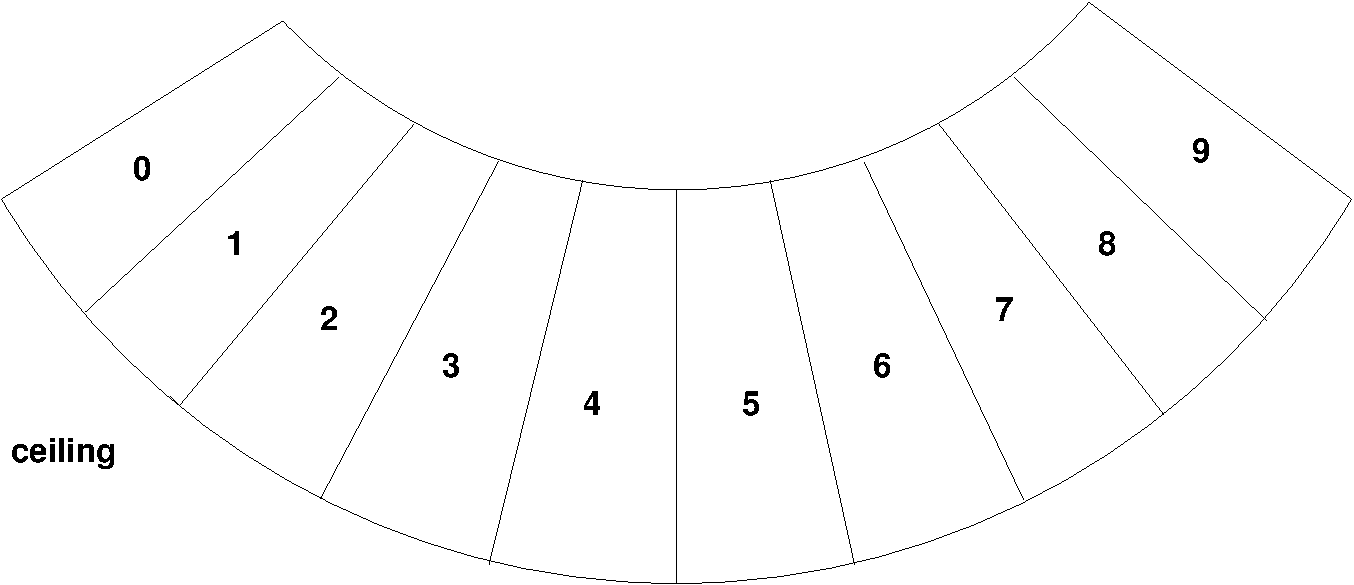
\includegraphics[width=5in]{ceiling.pdf}
\end{center}

\begin{center}
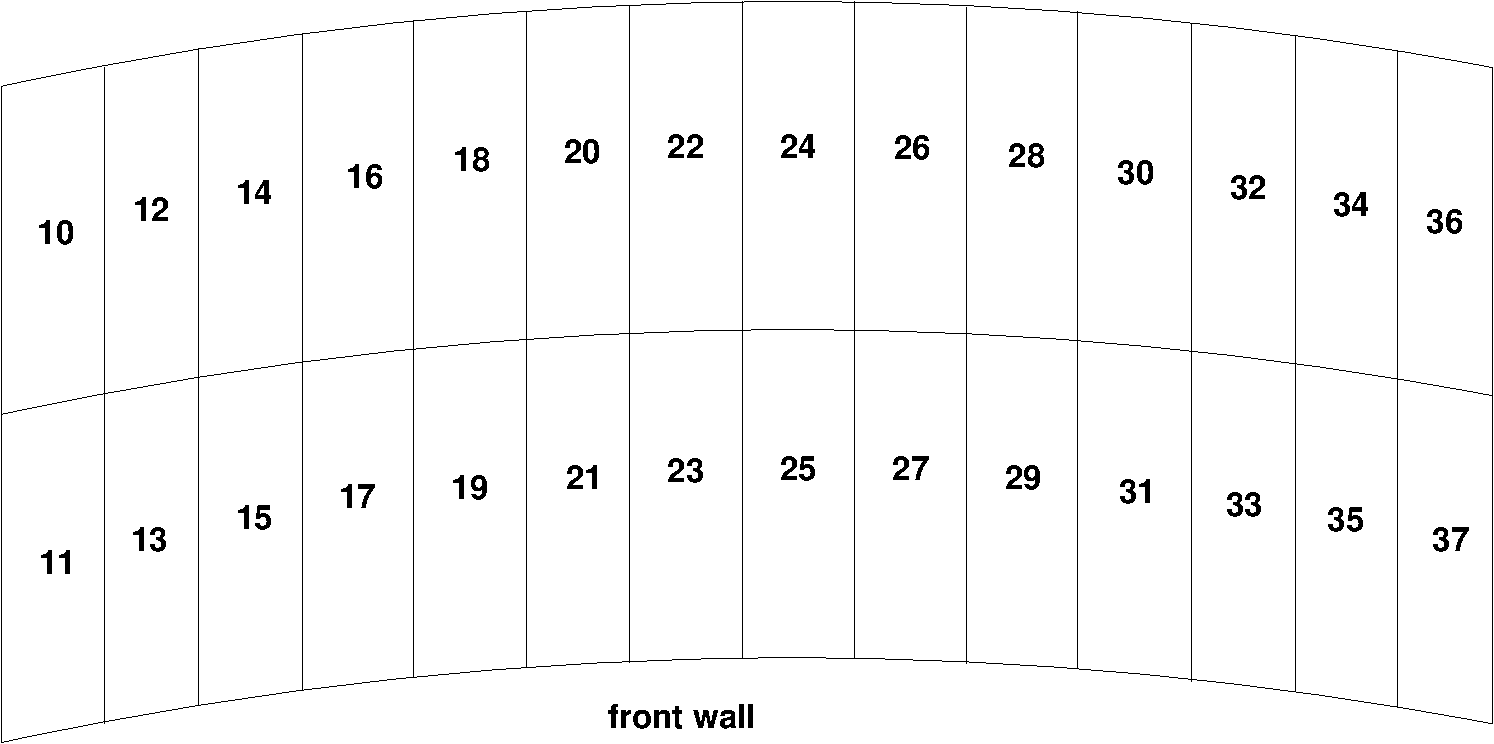
\includegraphics[width=5in]{wall.pdf}
\end{center}

\begin{center}
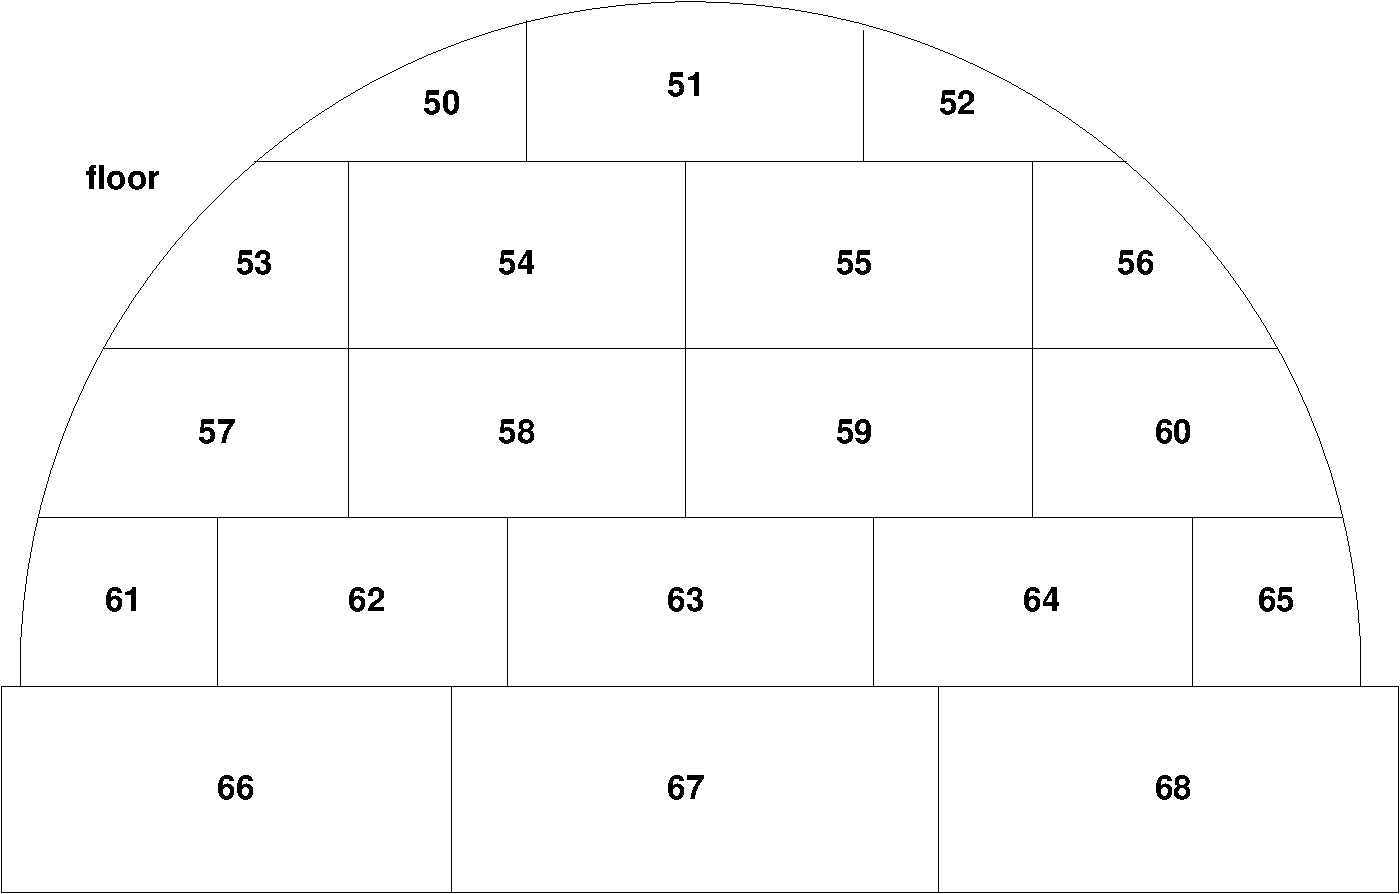
\includegraphics[width=5in]{floor.pdf}
\end{center}

\begin{center}
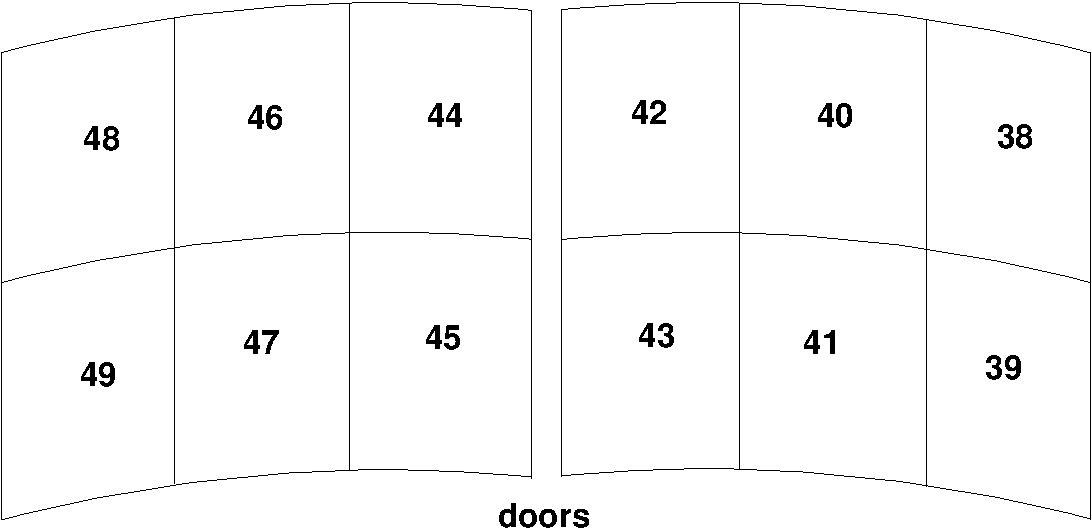
\includegraphics[width=4in]{doors.pdf}
\end{center}

\subsection{Operation}
\label{projector-operation}

Turn projectors on and off with the pjcontrol command.  
The pjcontrol command also is used to configure the projector color
and brightness, and to log repairs and track inventory.  The pjcontrol
script is part of the \cmd{cave-utils} module.  Load this with:

\begin{verbatim}
$ load module cave-utils
\end{verbatim}

You can see a help message with \cmd{pjcontrol \longcommand{help}}.  

\subsubsection{pjcontrol}

Synopsis:

\begin{verbatim}
pjcontrol.py [-h] [-s [SERIALNO]] [--clearErrs] [-d [MFGDATE]] [-a]
             [-R] [-G]
             [-r [{none,bulb,ballast,lens,board,install,uninstall,ship}]]
             [-l [{none,long,short}]]
             [-p [{none,spare,broken,installed,returned}]]
             [-c [COMMENT]]
             [projs] ...
\end{verbatim}

The pjcontrol script has two forms of usage, reference by projector
number, and reference by serial number.  Reference by projector number
looks like the following.   

\begin{verbatim}
$ pjcontrol projs command
\end{verbatim}

You can identify a projector by number individually, or in a list or
range:

\begin{verbatim}
$ pjcontrol 53 on
$ pjcontrol 33,34,35 on
$ pjcontrol 33-35 off
\end{verbatim}

The commands available are in the list below.  Unique abbreviations
are allowed. Some of these arguments require further args. For example
'install' requires a serial number, switch name and port, and
location. And 'repair' needs a serial number.

\begin{description}
\item[on] Turns projector on.  No arguments.

\item[off] Turns projector off.  No arguments.

\item[power] Returns the power status (0 = standby, 1 = warm up, 2 = imaging,
3 = cooling, 4 = error)

\item[version] Returns a software version string for the projector firmware.

\item[mode] Return the operation mode (0 = mono, 2 = stereo)

\item[mono] Set the operation mode to mono (s3d.mode = 0).

\item[stereo] Set the operation mode to stereo (s3d.mode = 2).

\item[lamp] Return the lamp mode (0 = standard, 1 = economy).

\item[eco] Set the lamp mode to economy.

\item[std] Set the lamp mode to standard.

\item[hour] Return the lamp hour counter value.

\item[error] Print the error log.

\item[raw] Send a raw command to the projector.  See the projector
  manuals for a list of the commands.  A command like the following
  sets the red gain to 125.

\begin{verbatim}
$ pjcontrol 13 raw red.gain = 125
\end{verbatim}
  
\item[repair] Log a repair.  (Please just use a single projector
  number for this command.)  This command needs a repair type and a
  double-quoted comment.

\item[install] Install a projector at a given switch location.  Use it
  like this when you're replacing a projector:

\begin{verbatim}
$ pjcontrol 42 install WACY00041
\end{verbatim}
  
  Use it like this if you have to replace the switch names as well:

\begin{verbatim}
$ pjcontrol 42 install WACY00041 switch03 1014 wall
\end{verbatim}
  
 Where the three additional arguments represent the name of the serial
 server switch, the number on the serial server that connects to the
 right projector, and an arbitrary screen name.


\item[uninstall] Takes a serial number.

\item[report] Provide a report (from the projector database.

\item[gather] Gather the variables that will be sued in a report.


\end{description}

Reference by serial number looks like this:

\begin{verbatim}
$ pjcontrol -s WACY00060 -r "bulb" -c "replaced bulb with s/n WYL889214"
\end{verbatim}

Note that you cannot reference multiple projectors by serial number
wild cards.  The serial numbers may be parial.  The projector
referenced with a partial serial number is the first one in the list
that matches the given fraction of a number.

\begin{description}
\item[-h, \longcommand{help}] Show a help message and exit.
\item[-s \argle{SERIALNO}, \longcommand{serial} \argle{SERIALNO}]
                        A projector serial number (or fraction
                        thereof).
\item[\longcommand{clearErrs}]   Clear the error log for a projector.
\item[-d \argle{MFGDATE}, \longcommand{date} \argle{MFGDATE}]
                        The projector serial number stickers have a
                        manufacturing date on them. Record it here, in the
                        format 2012-04-17.
\item[-a, \longcommand{add}] Add a projector to the
                        database. Requires that you specify a serial number
                        and date and optional lens type, and nothing else.
\item[-R, \longcommand{report}]     Produce a summary report about a projector. Without a
                        serial number specified, produce a summary report
                        about all projectors and all projector controls.
                        Ignores all other arguments.
\item[-G, \longcommand{gather}]    Run through all the projectors gathering all their
                        data. Ignores all other arguments.
\item[-r \argle{REPAIRTYPE}, \longcommand{repairType} \argle{REPAIRTYPE}]
                        Records a repair. Use this to
                        specify the type of repair, and do not forget to
                        include a comment.  The possible repair types
                        are bulb, ballast, lens, board, install,
                        uninstall, ship.  You can also use ``none'' to
                        insert a comment into the repair log.
\item[-l \argle{LENSTYPE}, \longcommand{lens} \argle{LENSTYPE}]
                        Sets type of lens (long, short, none) for the given
                        serial number.
\item[-p \argle{PURPOSE}, \longcommand{purpose} \argle{PURPOSE}]
                        Record the current purpose of the projector (spare,
                        broken, installed, returned).
\item[-c \argle{COMMENT}, \longcommand{comment} \argle{COMMENT}]
                        Commentary about the repair.  Must be quoted
                        if it contains more than one word.

                      \end{description}
                      
\subsubsection{pjlog}

The pjcontrol command logs its usage at cave-utils/yurt/log.
You can see the last few log entries with the pjlog command.

\subsubsection{pjreport}

Creates and stores a full report of the state of the projector
database.  This should be run at least weekly.

\subsubsection{projd}

In order to address deficiencies in the Scalable Display Manager
software, there is a system by which projector commands can be sent to
an IP address, and forwarded to a specific projector.  The projd
command listens on a set of ports, and forwards the connections to the
projector correponding to that port.

The projd script calls the projd.py Python script, which defines a
projChats object that takes two numbers as an argument:

\begin{verbatim}
projChats(address, projector)
\end{verbatim}

Where \cmd{address} is the last segment of an IP address that begins
with 192.168.160. and projector is the number of the projector to be
controlled at this address.  The projd.py command uses the
pjcontrol-raw script, which is not to be used otherwise.

\subsubsection{pjexpect}

This is part of the pjcontrol script operation and is not meant to be
used independently.


\subsection{Inventory and Logs}
\label{logging}

The projector database is currently held in the etc directory of the
cavedemo account.  It is an anydbm file, readable with the pjcontrol
python script stored in the cavedemo bin directory.

\begin{verbatim}
$ /users/cavedemo/bin/pjcontrol -R
\end{verbatim}

This produces a report of the condition of all the projectors, and a
list of all the installed projectors.

The following commands will produce a report about a single
projector.  The first will only work on an installed projector, while
the second will work on any projector in the database.

\begin{verbatim}
$ pjcontrol 53 report
\end{verbatim}

\begin{verbatim}
$ pjcontrol -s WOCY00022 -R
\end{verbatim}

\subsubsection{Periodic logs}

The pjcontrol system should have all the error and color calibration
records updated periodically.  Run:

\begin{verbatim}
$ /users/cavedemo/bin/pjcontrol -g
\end{verbatim}

This steps through all the projectors, downloading their error
record, color calibration, and usage time data into the master
database.

\begin{note}[IMPORTANT]
This is only effective when all the projectors are turned on.
\end{note}

This should be run weekly, with a report run and recorded as often.
Use \cmd{pjreport} (with no arguments) to create and store a report for
the current date and time.

\subsection{Maintenance and repairs}

So far as we currently understand it, the only maintenance required is
the replacement of bulbs.  Policy is to replace them when they blow
out, not to anticipate their demise.

All maintenance and repair actions should be recorded on the paper
maintenance log.  The actions relevant to a specific projector will be
entered into the projector database from that record, by Tom.  (You
are welcome to enter them yourself with the pjcontrol script.  Please
record on the paper log that it was successfully entered.  See
section~\ref{logging}.) 


\subsubsection{Bulbs}

Bulbs should be replaced when they blow out.  We are not currently
replacing them proactively.  Once the color calibration is functional,
we will be keeping data about color change over the bulb lifetime and
may change policy after analyzing that data.

We are currently procuring bulbs from the manufacturer, but we have
identified two alternate bulb suppliers at present:

\begin{description}

\item[Relampit] Contact: Tom Sullivan, Relampit, 120 Wilbur Place, Suite C,
Bohemia, NY 11716, 631-244-0051x122, tsullivan@relampit.com, \$558
new, \$495 relamp.  Warranty runs 90 days from installation, free
shipping.

\item[Greenleigh and Wong] Contact: Tom Greenleigh, Greenleigh Wong Lamps, 1680
Navajo Road, Ground Floor, Ogden UT, 84403, 801-475-7800,
tom@gwlamps.com. \$535 new, \$361 relamp.  Warranty runs 180 days from
shipping.

\end{description}


\subsubsection{Shipping for repair}

Units should be shipped for repair in one of the original boxes. There
are a few still around.

Before sending off, please ensure that the error record of the
projector is recorded in the projector database. If the projector is
not currently installed, do this by installing it at port 70 (the
repair port), and issuing the following:

\begin{verbatim}
$ pjcontrol 70 gather
\end{verbatim}




\subsection{Ventilation}

The wall projectors are vented directly into the AC return duct at the
back of the room.  It is important to make sure the lowest extension
of the duct is blocked.

Where is the system controlled?  How?  Does it change with the
heating/cooling season?

1) how can the cooling system be monitored so that problems with it
don’t lead to projector damage

2) is the return booster operating?  How can we tell, and how do we
turn it on if it isn’t on

3) the makeup air intake through the roof will potentially mix in
outside air, potentially reducing the return flow.  How do we ensure
that doesn’t cause problems with this system that is cooling both
people space and equipment?


\subsection{Frame Lock}
\label{framelock}

Sometimes the projectors get out of sync with each other, and the
stereo is different every way you look.

The projectors are synchronized electronically with daisy-chain
connections among the cave nodes which serve to synchronize the
graphics cards.  The settings do not persist through a restart of the
cave X servers (which includes power interruptions or reboots).  Use
this procedure to reset the frame lock.

\begin{enumerate}

\item Log in as cavedemo.  Use one of the linux terminals in the lab,
  or ssh -X to one of the cave nodes.

\item Run \cmd{nvidia-settings -c cave001:0}.  This should start up
  a GUI for you.

\item In the left pane of the window, look to the bottom for
  ``framelock'' and click that.  You should see a long list of
  projectors appear in the main window.

\item Look in the bottom right of the window for a ``disable frame
  lock'' button.  Click it, wait, then click ``enable frame lock.''
  You'll see lots of green if it worked.

\end{enumerate}


The nvidia-settings program is initialized with a startup file called
\cmd{.nvidia-settings-rc}, currently in the cavedemo home
directory.  We have not had good results editing this file directly;
editing configuration should be done with the GUI.


\section{Tracking, Heads and Pointers}

\subsection{Opti-Track tracking system}
\label{opti-track}

\begin{note}
  The Scalable calibration display clients occasionally seem to affect
  the sync signal received by the opti-track software.  You may have
  to restart the framelock after calibrating the projectors.  See
  section~\ref{framelock}.
\end{note}

The Opti-Track system consists of a bunch of cameras aimed at a bunch
of reflective balls.  When three or more cameras see a particular
ball, they can pinpoint its position to within a millimeter.  When the
cameras see three out of some random constellation of balls, such as
is on the tracked glasses, or the wand, the system can pinpoint that
constellation and thus the gaze or the hand of the user.


\begin{note}
  The Opti-Track license dongle seems to interfere with the booting of
  the kiosk machine.  Remove the dongle to reboot and reinsert it when
  the computer is safely up and running.
\end{note}

\subsubsection{Starting the Opti-Track}

Double click on the ``Motive'' software icon.  When it comes up it
will ask whether you want to open an existing project.  Say yes, and
then choose the ``Cave'' project, usually at the bottom of the list.

\subsubsection{Calibrating the Opti-Track}

To calibrate the Opti-Track system, start it up as above, then click
``Layout'' and choose the calibration option from the drop-down menu.

\begin{enumerate}

\item Mask the visible light sources.

\item Choose calibration type (``full'') and `optiwand' option
  (``large''). 

\item Make sure that all the cameras are accounted for and reporting
  properly in the list on the left of the window.

\item Click ``start wanding'' and start waving the wand around slowly
  up and down.  The cameras have some feedback capacity built into
  their lights.  You'll see the cameras near you turn green as they
  are satisfied, then move over nearer another not-yet-green camera.

\item Eventually the software will tell you it has enough data for a
  good (or very good) calibration, at which point you can stop.

\item Click ``calculate''

\item Set the ground plane thing on the floor.  The origin of the cave is on
  the seam of the true floor (not the sacrificial floor), halfway
  across.  Put the ground corner of the ground plane over that point,
  and aim the long leg at the center of the screen.  Level it if
  necessary.

\item Click ``ground plane''

\item The actual zero of the \yurt is four feet above the ground plane,
  so you'll have to adjust the Y dimension of the calibration to equal
  -1219 (millimeters).  You should see the lighting icons drop down in
  the display pane.

\item Click on the file menu, and save project.

\end{enumerate}


\subsubsection{Adding an object to the calibration}

The glasses and wand are constellations of reflectors whose pattern is
stored and recognized by the Opti-Track software.  Sometimes you'll
want to replace these items, or the metal may become bent and the
system will not recognize it any more.

To replace an object in the calibration, click on the project
description, then

Steps for adding/replacing an object.


\subsubsection{3D printer patterns}

There are a variety of 3D print patterns for various \yurt accessories
found in the cavedemo data directory, in the \cmd{yurt-tools} directory.


\subsection{Polhemus tracking}

The Polhemus (magnetic) tracking system is not currently installed.

% Charging, location of transmitter, how is it connected and powered?

% Is there software that needs to be started/restarted?

\subsection{Pointer}

The location of the wand is controlled by the Opti-track software, but
the button presses and joystick operation takes a different route.

The wand communicates with the system via a dongle on the kiosk
computer.  If the wand's VRPN server is running, the button presses
are reported as VRPN events, using the key below.

\begin{center}
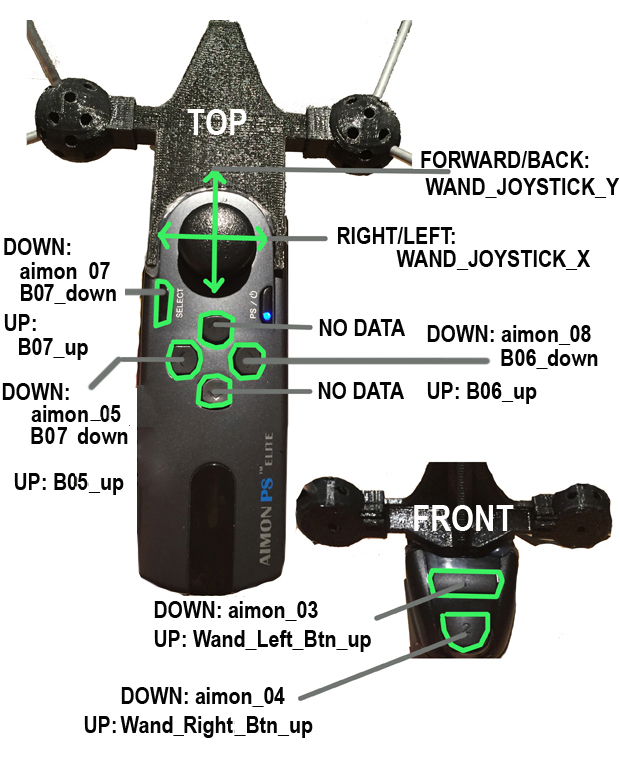
\includegraphics[width=0.6\columnwidth]{yurt-wand-controller.jpg}
\end{center}

Don't forget to restart the wand's VRPN server if the dongle gets unplugged.


To plug in the dongle, look for a small button on its end.  Press the
button while inserting the dongle into the kiosk computer's USB port.

Wand must sometimes be ``paired'' with the dongle.  Sometimes this
happens on battery changes, and it definitely happens when the wand is
swapped for repair.  The wand will complain that it is not paired by
flashing its blue power light.  To pair, press the button on the
dongle and within eight seconds, press both the power button and the
select button (the button opposite the power button on the wand).  This is an
undocumented feature of the wand, so these instructions are merely
provisional, but this appears to work.


\section{Glasses, Stereo}

The Volfoni glasses are operated by an RF signal generated by a small
transmitter plugged into the sync output of projector 11.  (Bottom
left on the front wall.)  It is powered by a controllable plug strip,
so that it can be turned off then the \yurt is not in use.  This allows
the glasses to time out and power down.


\subsection{Stereo backwards}

There is currently no positive identification of the left and right
eye in the stereo signal.  Sometimes when the system is started
up, the signals will be swapped and the stereo will appear wrong, with
the viewer's left eye shown the image that belongs on the right.
Worse, the stereo polarity is known to spontaneously reverse from time to
time.  This is irritating and we are working on fixing this problem.
In the meantime, to fix the problem, you can use the controls for the
Opti-Track software.  (See section~\ref{opti-track}.)

Over on the right hand side of the Motive software window, you'll see
an ``Output 1'' list of attributes.  Beneath it, there is a
``Polarity'' setting, with a dropdown menu.  Click on that option,
change the polarity from inverse to normal or the other way around,
and click ``Apply'' at the top of that column of the screen.


The kiosk has a program on it for checking the stereo configuration
(on the System tab).  It alternates red and green fields for the left
and right eyes.  When you hold the glasses up against any part of the
\yurt screen, one lens will appear red and the other green.  When the
glasses look like the image of the glasses in the icon, the stereo is
configured correctly.  

When the framelock is not working, there will frequently be areas of
the screen for which the stereo is not working.  If you see
inconsistencies across the field of view, try resetting the
framelock.  See section~\ref{framelock} on Framelock. 


\iffalse

You can also toggle the stereo by turning projector 11 stereo off and
then on again.

\begin{verbatim}
$ pjcontrol 11 mono
$ pjcontrol 11 stereo
\end{verbatim}

There is only a 50\% chance that this procedure will leave the system
in the correct state, so you may have to try it a few times before it
works properly.  Take comfort in the fact that there is only a 6.25\%
chance you'll have to do it more than four times.

\fi

\subsection{Operating the glasses}

To turn the Volfoni glasses on, press the button (not the switch) on
the left temple.  You'll see the lenses blink left, then right, then
wait a beat, and both lenses will go dark together.  When you put the
glasses on you should see the stereo images.

The switch on the glasses does not do
anything.  (Except on one pair somewhere, where it reverses the
stereo.  That pair is marked with an `M' on the temple.)

If the glasses are on, pressing the button will cause the LED on the
bridge of the nose to blink.  Three blinks mean fully charged, two
means sort of charged, and one blink means charge me.

The glasses will not turn themselves off as long as the RF transmitter
is within range.  Since it covers the room, assume the glasses do not
turn themselves off.  To power off the glasses, hold the button down
until the lenses go clear.

\section{Kiosk and Demos}

The Kiosk is (sadly) a Windows machine.  There isn't a lot to say
about it, but when it misbehaves and needs to be rebooted, use this
procedure.

\begin{enumerate}
\item Remove the Opti-Track software dongle from the USB ports on the
  back.  Remember which port it came from.  This dongle appears to
  prevent the machine from booting properly.

\item Reboot.

\item Replace Opti-Track dongle.

\item Restart tracking, pointer, and sound server software.

\item Start Internet Explorer and make sure it's pointing at the Kiosk
  web page.

\end{enumerate}

The kiosk itself is a web page, hosted on dev09.
% the virtual host caveweb1.oscar.ccv.brown.edu.

\subsection{Demos}
\label{Demos}

Many of the demo programs use data assumed to be in the
\cmd{/tmp/yurt-data} directories of the cave nodes.  There is a
model directory in the cavedemo account, see
\cmd{/users/cavedemo/data/model\_tmp}.  You can copy the
\cmd{model\_tmp} directory contents to the node
\cmd{/tmp/yurt-data} directories with the
\cmd{copy\_data\_to\_tmp script} in the.


\section{Scalable software, Warping and Blending}

Software from Scalable Display manages the blending and warping of the
projector images so that several projectors can work as one.  This is
commercial software, with a license that must be kept up to date.
Also, the system must be recalibrated periodically, as projectors are
jostled or vibrate to a different position.

\subsection{License}

The scalable license file should be kept in the cavedemo z: folder,
under the \cmd{scalable} directory.  Look for a .licx file.

\subsection{Calibrating the software}

Calibrating a wall of the \yurt involves pointing a camera at the wall
and running the calibration software.  The software illuminates the
projectors one at a time, and notes its position, including the edges.
This is used to calculate the zones in which the projector images
overlap.

\subsubsection{Running calibration}

These are the steps for running a calibration.  The projectors should
be calibrated periodically, as well as after any work that might
involve jostling or moving them.  The calibration is done per wall.
There are five walls in the syste: front, ceiling, floor, left and
right doors.

\begin{enumerate}

\item Turn on relevant projectors, plug in camera.  Make sure the camera
  appears as a USB device on the console computer.  Set up the camera
  so it is looking at the wall to be calibrated.  The camera should be
  set on Manual exposure.\footnote{The camera occasionally loses the
    connection with the Windows machine.  You'll know when the
    Scalable Display Manager fails to operate the camera shutter.  At
    the moment, there is no known cure besides rebooting the kiosk
    machine.} 

\item Start Scalable display clients on each of the relevant nodes.
  This is done by executing RunDisplayClient.sh on each node.  For
  convenience, there is a ``Calibrate'' icon in the System window of
  the kiosk that will start the display clients on all the nodes.

\newcommand{\bs}{$\backslash$}
\item The configurations are kept on the kiosk machine, in zip files
  within the directory \hbox{\cmd{C:\bs cave\bs scalable\_configs}}.  You will find several zips in
  there, called \cmd{DefaultSystem\_Ceiling.zip} and so on.  These need to be
  unpacked into \hbox{\cmd{C:\bs Program Files\bs
      ScalableDisplay\bs DEI\bs SystemData}}.  On the kiosk Desktop,
  you'll find a \cmd{Scripts} directory with clickable Windows scripts
  you can use that will unpack the right zip file for you.  Click on
  the appropriate one of 
  those scripts to copy all the calibration files into the right
  place and start up the Scalable Display Manager.

\item With the SDM running, use the ``Display Clients'' tab to choose
  which display clients you are talking to.  Check that the clients
  used by the screen you are calibrating are 
  green and on the right. 

  \begin{center}
  \begin{tabular}{ll}
    Front wall & cave001, cave002, cave003, cave004, cave005, cave006,
                 cave007 \\
    Ceiling & cave008, cave009, cave010 \\
    Left door & cave011, cave019 \\
    Right door & cave012, cave013 \\
    Floor & cave014, cave015, cave016, cave017, cave018 \\ 
  \end{tabular}
\end{center}

The display client window does not scroll.  If you don't see the right
client on the left-hand list, you can specify the IP address directly
into a box in the right column.  The Display Client nodes you want are
numbered 172.20.160.X, where X is the number of the cave node.

\item ``Projectors'' display.  Your projectors should be in a 1xn row in
  order to make the calibration cursors appear in a later step.  All
  the projectors you see should have the little box checked.  Click
  ``Next'' in the lower right corner, and move on to the camera
  display.

\item ``Cameras'' display.  Set the exposure for the camera down to about
  .25s, then click on ``Begin Data Collection'' and watch the (not very
  interesting) light show.  The computer will turn on each projector
  full white, then go back and do them all with little blocks, and
  with a central image that defines the orientation of the
  screen.  Click ``Next'' in the bottom right corner to advance.

\begin{note}
  When calibrating the ceiling, you will need to do it twice.
  Calibrate the ceiling up to this point (including the ``Update
  Calibration'' button on the next page), and then run the
  ``Create\_Ceiling\_Masks'' script in the Desktop ``Scripts''
  directory and do the ``Cameras'' step again.
\end{note}

\item Screens tab.  Use this to confirm the shape of the screen looks
  more or less the way you anticipate it will look, and then click
  ``Next'' and move on.

\item ``Image Boundary'' tab.  Use this to set the control point
  positions for the calibration.  There are two methods, the first
  involving moving cursors around the screen itself, and the second
  looking at a camera image of the screen.  To use the camera method,
  go back to the Camera tab, and increase the exposure time of the
  camera (about 5 seconds works well) then come back to this tab and
  select ``Pick boundary points within camera images.''  Use the mouse
  to drag the control point positions onto the screen image.

  For the ceiling calibration, this is probably the preferred method,
  since the outside control points at the top of the screen (numbers 1
  and 3) seem best when located a few inches outside the physical
  screen.  (That edge of the screen is convex, so if you put the
  points exactly on the screen corners, the outside edge has no image
  on it halfway between the corners.)

\item To use the cursor-on-wall method, click ``Position points along
  screen boundary.''  Click on each of the points, and maneuver it
  into place by either dragging with the mouse or using the arrow keys.

  \begin{description}

  \item[Front wall] Six control points, four on the outer corners, and
    two at the center, at the top and bottom edges.  The center isn't
    spiked just now, but should be.

  \item[Floor] Four control points, two are placed where the floor
    seams meet the front wall, and the other two are placed at the
    floor corners, just past the wall edge.

  \item[Doors] Place the control points at the four corners.

  \item[Ceiling] Six control points, four on the outer corners, and
    two central.  The center isn't spiked, but should be.

  \end{description}

  If the control points are placed in some way that the software deems
  impossible (maybe you have the order incorrect, for example), the
  software will respond with an error 79, and an incomprehensible
  message about not being able to write the ScalableDisplay.ol0 file.

\item Perspective display.  All the walls are defined with coordinates
  that place them in the front of the room.  After calibration, these
  shapes must be rotated into the correct location.  The ``Eye Point''
  menu in the perspective display is where this rotation happens.
  This has been set already, and if you are using the proper
  ``DefaultSystem'' directory, you should not have to reset this.

\item After the control points have been placed, you can click
  ``update calibration'' and if it runs successfully you're done with
  the hard part, congratulate yourself.

\item After successful calibration, the output POL files must be
  renamed and distributed to their final locations.  There are a set
  of scripts in the cavedemo directory \cmd{winders/cave/scripts}
  called \cmd{copy\_front.sh} and the like.  These are to be executed in
  a cygwin window on the kiosk (Windows) machine, where they can be
  found at \cmd{/cygdrive/z/winders/cave/scripts.}

\item Backup a successful calibration by running the script (in the
  same directory) called \cmd{backup\_front\_wall.sh} and its friends.
  Run in the same manner as the copy script above.


\end{enumerate}

\begin{note}
  The calibration display clients seem to affect the sync signal
  received by the opti-track software.  You may have to restart the
  framelock after calibrating the projectors.  See
  section~\ref{framelock}.
\end{note}




File locations for the display clients are controlled on the
``Advanced'' options page of the Display Manager.

Most times you will not need to adjust any of these settings.  They
are recorded here in case something goes wrong.

\begin{enumerate}
\item obj file is in DEI/SystemData/DefaultSystem/Config,
  ControlPoint3DLocationOverride contains the coordinates of the
  control points.

\item Things to configure: RemoteOutputDirectoryName (directory only),
  also Perspective SDK Mesh File Output Path and Orthographic [same].
  Last two are complete path and file names.  These are redundant with
  the remote output directory name, but need to be set redundantly.
  [THIS DOES NOT SEEM NECESSARY]

\item Camera settings: ISO 200, .125 sec, f/11.

\item C:ScalableDisplay/ScalableServiceInformation has jpegs in it for
  each projector.

\item There is a mask available for the calibrating.
\end{enumerate}








\subsubsection{Digest camera data}

\subsection{Location of POL files}

The installed POL files (the output of the Scalable calibration step)
are located in the cavedemo account home directory, in
``/users/cavedemo/scalable/cave.''


\subsection{Scalable libraries}

Pointer to Scalable documentation?

mgt.oscar.ccv.brown.edu


\subsubsection{Making a model}

What constraints on the model?

via blender, via kinect?

On Win machine, logged in as last mohican (hawkeye), there is said to
be a file with a modest amount of documentation about how to use and
install obj files.  Lies, all lies!


\subsubsection{Importing the model}

How to get it read by the Scalable Display manager thing.

John's zipfile hack.


ScreenTypeOverride


\section{Software}

Libraries, APIs,


\section{Construction}

Knot for tying monofilament, ``Nanofil''

Mirror suppliers



\section{Granoff Cave}

This section of this document is about the old VR installation, herein
called the ``cave''

\subsection{Startup}


Start the various servers from the start menu, not from the desktop.

The VRPN server will start up, but might not start sending frames if
an OpenGL program is not running somewhere.  Try starting it while the
``Align Screen'' (a simple OpenGL program that uses no input)
application is running.


\subsubsection{Frame lock}

On a restart, you should check to see if the frame lock is still set.
Log in to the caveserver as cavedemo, start nvidia-settings -c
cave5:0, and then add cave5 in the framelock panel.   See
  section~\ref{framelock} for more.

\end{document}
